While a program is running, a statement or expression may cause an error.
These errors are called \textit{exceptions}. In Python, exceptions are objects that a program can manipulate.
You've probably seen many exceptions already, since most aren't handled by programs.
\vspace{0.5mm}
\begin{lstlisting}
>>> '1' + 1
Traceback (most recent call last):
  File "<stdin>", line 1, in <module>
TypeError: can only concatenate str (not "int") to str
\end{lstlisting}
Here, the first line of the error is the traceback, which shows where the \lstinline{__context__} where an error occurred.
The kind of exception, in this case a  \lstinline{TypeError}, can vary depending on the cause.
The last line of the error message is the \lstinline{value} of the exception and explains what happened.


There are many kinds of exceptions! The chart below shows just a few of them, see you if you recognize any.
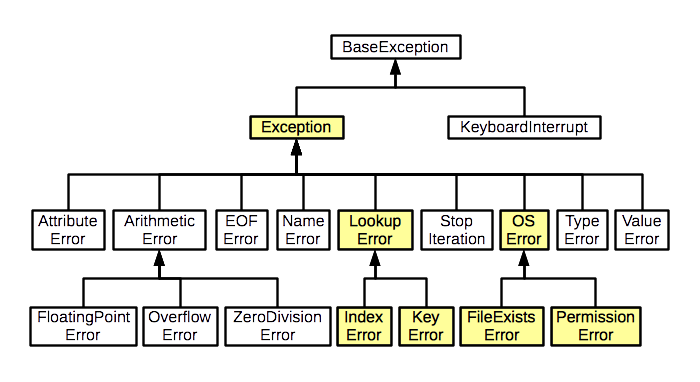
\includegraphics[width=\textwidth]{exceptions-hierarchy.png}

Now, suppose you wish to raise your own custom exception.
You can create a new exception by calling the \lstinline{Exception} constructor and passing in the error message as the value.  
To raise the exception (and interrupt the code), use the \lstinline{raise} statement.
\begin{lstlisting}
    >>> raise Exception('An error occurred')
    Traceback (most recent call last):
    File "<stdin>", line 1, in <module>
    Exception: an error occurred
\end{lstlisting}

You can also use the \lstinline{assert} statement to raise an \lstinline{AssertionError}.
\begin{lstlisting}
    >>> assert 4 > 5
    Traceback (most recent call last):
    File "<stdin>", line 1, in <module>
    AssertionError
\end{lstlisting}

However, your code doesn't need to fully crash when an exception is raised.
We can "handle" exceptions with a \lstinline{try}-\lstinline{except} block in the following format.
\begin{lstlisting}
    try:
        <try suite>
    except <exception class> as <name>:
        <except suite>
    ...
\end{lstlisting}
We can have as many \lstinline{except} clauses as we would like. This is the corresponding behavior when running this block:

\begin{enumerate}
    \item Python runs the \lstinline{try} suite.
    \item If it encounters an Exception during this, it interrupts the \lstinline{try} suite.
    \item Python finds the first \lstinline{except} block which corresponds to the class of the exception.
        \begin{itemize}
            \item If no such \lstinline{except} block is found, the exception is not handled.
        \end{itemize}
    \item If Python can find a corresponding block, the exception object is bound to \lstinline{<name>}, and the \lstinline{except} block is run.
\end{enumerate}

Note that if we just use \lstinline{except} by itself, it just catches any possible Exception. Generally, this is bad practice and shouldn't be used.

Here is an example of how we can handle exceptions.
\begin{lstlisting}
    >>> try:
            positions = {'peter': 'SCM', 'cyrus': 'SCM'}
            x = positions['josh']
        except KeyError as e:
            print('handling a', type(e))
            x = 'Coord'
    handling a <class 'KeyError'>
    >>> x
    'Coord'
\end{lstlisting}

\begin{blocksection}
\begin{guide}
\textbf{Teaching Tips}
\begin{itemize}
    \item Give examples for why raising an exception might be useful (RecursionError stopping our code from running forever, etc.).
    \item Give examples of handling exceptions (stopping edge cases like division by 0, etc).
\end{itemize}
\end{guide}
\end{blocksection}